\subsection{ACIM Parameter Estimation}

A Fluke energy analyser is used over regular analog meters for more reliable and accurate measurement of the voltage, current and active power. But, for low current and power measurements properly calibrated analog meters would suffice as the the energy analyser wouldn’t be able to measure currents less than one amp.

\subsubsection{Cold Test}

The stator resistance is measured by running the motor at its rated current for 5 minutes or up until it reaches its thermal equilibrium.


\subsubsection{No-Load Test}

% hardware setup for no-load test

\begin{figure}[H]
	\centering
	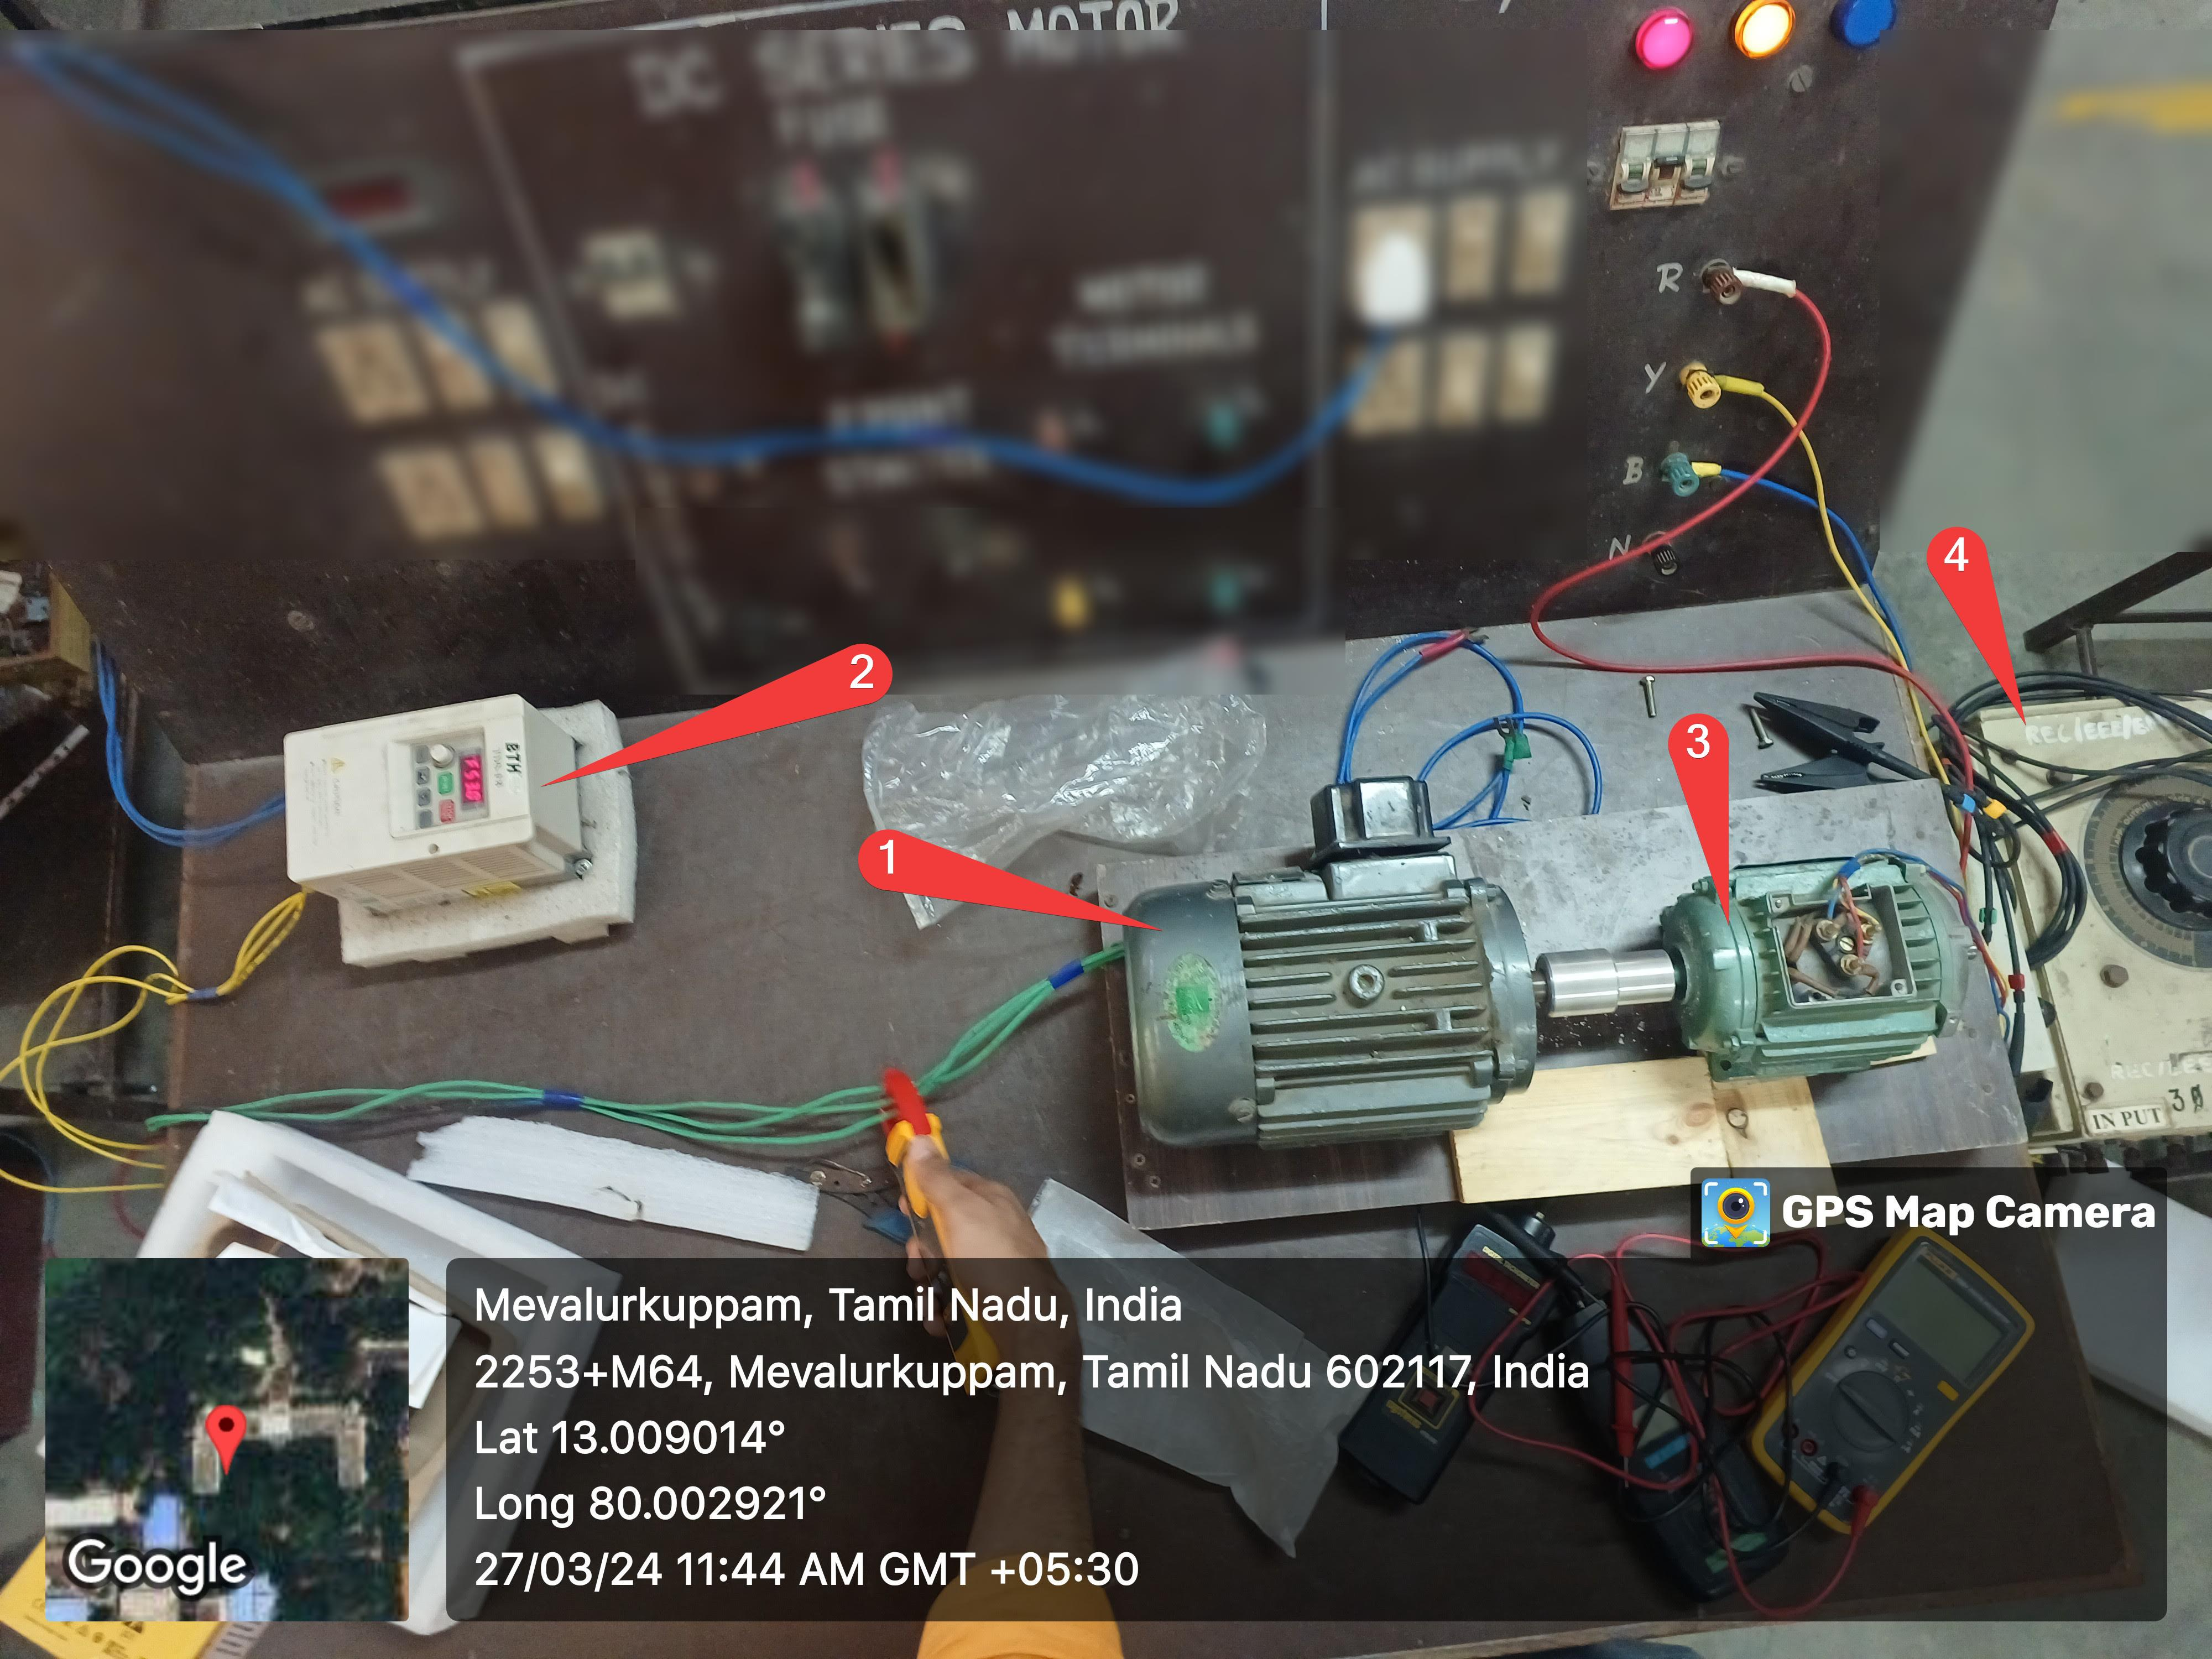
\includegraphics[width=4in]{sections/section5/images/ParamEstim/SetupNoload.jpg}
	\caption{No-load test setup}
	\label{fig:no_load_test_setup}
\end{figure}

The no-load setup has 1Hp induction motor connected to variable frequency drive (VFD) to supply no-load losses like friction and windage losses of 0.25Hp motor which is connected to the power analyzer as shown in \ref*{fig:fluke434}


% Fluke 434 analyzer image voltage amps hertz is shown in the figure

\begin{figure}[H]
	\centering
	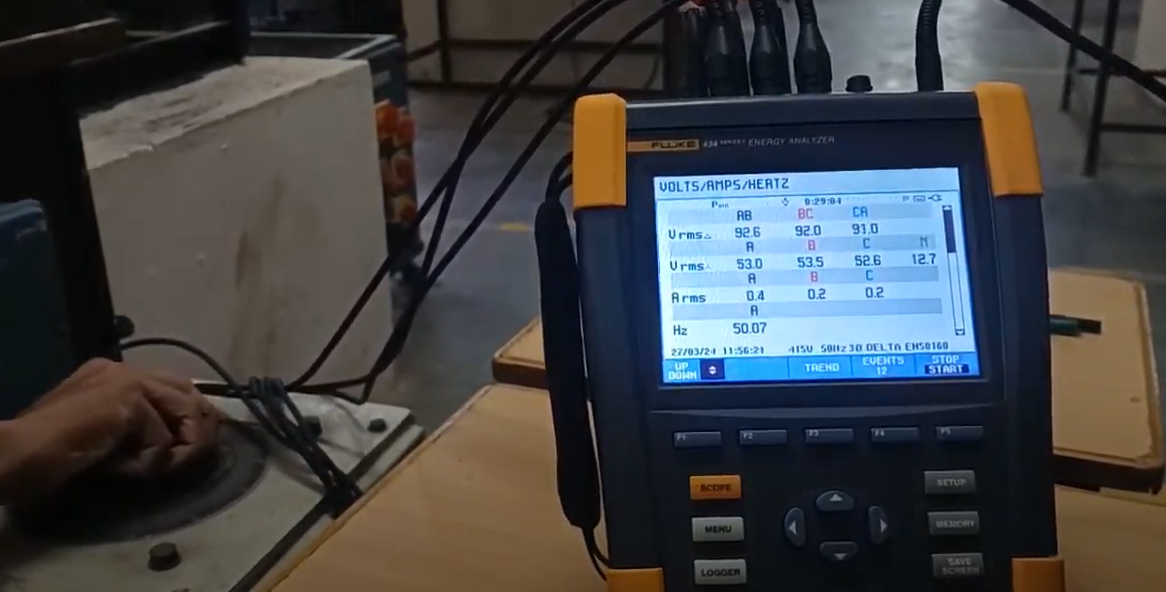
\includegraphics[width=4in]{sections/section5/images/ParamEstim/FlukeVoltAmpHertz.png}
	\caption{Fluke 434 power analyzer}
	\label{fig:fluke434}
\end{figure}

% From R Krishnan book circuit equivalent figure

\begin{figure}[H]
	\centering
	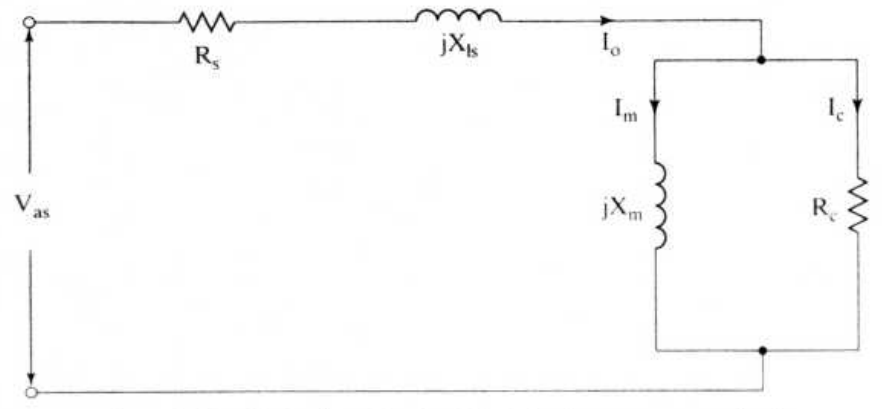
\includegraphics[width=4in]{sections/section5/images/ParamEstim/noloadCircuitKrish.png}
	\caption{No-load test circuit}
	\label{fig:no_load_test}
\end{figure}

The no-load power factor is given by:
$$\cos \phi_0 = \frac{P_i}{V_\text{as}I_0}$$

The magnetizing current is calculated as:
$$I_m = I_0 \sin \phi_0$$

The core-loss current is given by:
$$I_c = I_0 \cos \phi_0$$

The magnetizing inductance is computed from:
$$L_m = \frac{V_\text{as}}{2\pi f_\text{i}I_m}$$

The core-loss resistance is given by:
$$R_c = \frac{V_\text{as}}{I_c}$$


\subsubsection{BLOCKED Test}

% Blocked rotor circuit equivalent figure

\begin{figure}[H]
	\centering
	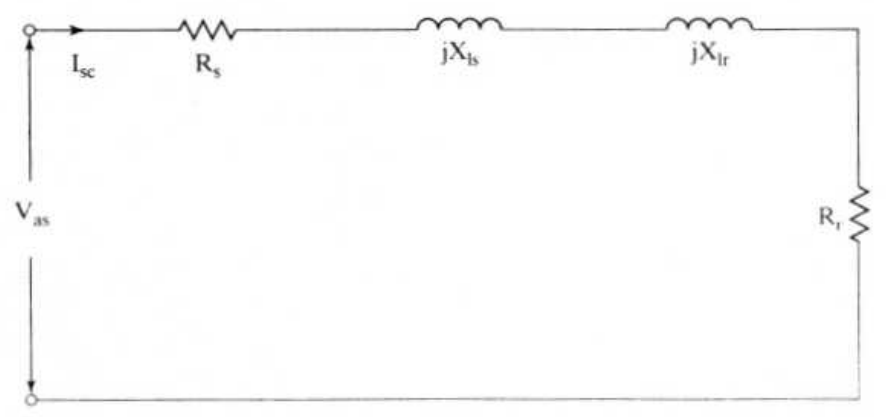
\includegraphics[width=4in]{sections/section5/images/ParamEstim/blockedCircuitKrish.png}
	\caption{Blocked rotor test circuit}
	\label{fig:blocked_rotor_test}
\end{figure}


The short-circuit power factor obtained from the equivalent circuit is:
$$\cos \phi_\text{sc} = \frac{P_\text{sc}}{V_\text{sc}I_\text{sc}}$$

The short-circuit impedance is given by:
$$Z_\text{sc} = \frac{V_\text{sc}}{I_\text{sc}}$$

From which the rotor resistance and total leakage reactance are computed as:
$$R_r = Z_\text{sc} \cos \phi_\text{sc} - R_s$$
$$X_\text{eq} = Z_\text{sc} \sin \phi_\text{sc}$$

where the total leakage reactance per phase, $X_\text{eq}$, is the sum of the stator and referred-rotor leakage reactances, given as:
$$X_\text{eq} = X_\text{ls} + X_\text{lr}$$



Based on the above test and calculations, the equivalent circuit parameters are computed as follows:

% Alighn left
\begin{flalign*}
	&L_m = 1.01 \, \text{H}, \quad R_c = 1555.85 \, \Omega                  &\\
	&R_r = 5.02 \, \Omega, \quad X_{ls} = 50.47 \, \Omega, \quad X_{lr} = 50.47 \, \Omega &
\end{flalign*}

\newpage